% 24th, Jan, 2001 Ver.1     Tatsuya Okabe
%                 Ver.2
%                 Ver.3
%                 Ver.4
%                 Ver.5
%
%---------------------------------------------------------------------------%
% Made by Tatsuya Okabe ( HONDA R&D Europe ( Deutschland ) GmbH )           %
% Checked by Bernhard Sendhoff ( HONDA R&D Europe ( Deutschland ) GmbH )    %
%---------------------------------------------------------------------------%
% Class NegExponential

\section{Abstract}

\noindent
With the class {\em NegExponential}, we can calculate the ``Negative
Exponential'' distribution with the following equation.

\begin{equation}
f(x) = \frac{1}{a} \cdot \exp\left\{\frac{-x^2}{a}\right\}
\end{equation}

\noindent
In this equation, $a$ and $x$ mean the constant value and the variable respectively.

\vspace*{10mm}

\begin{center}
\begin{figure}[h]
\rotatebox{-90}{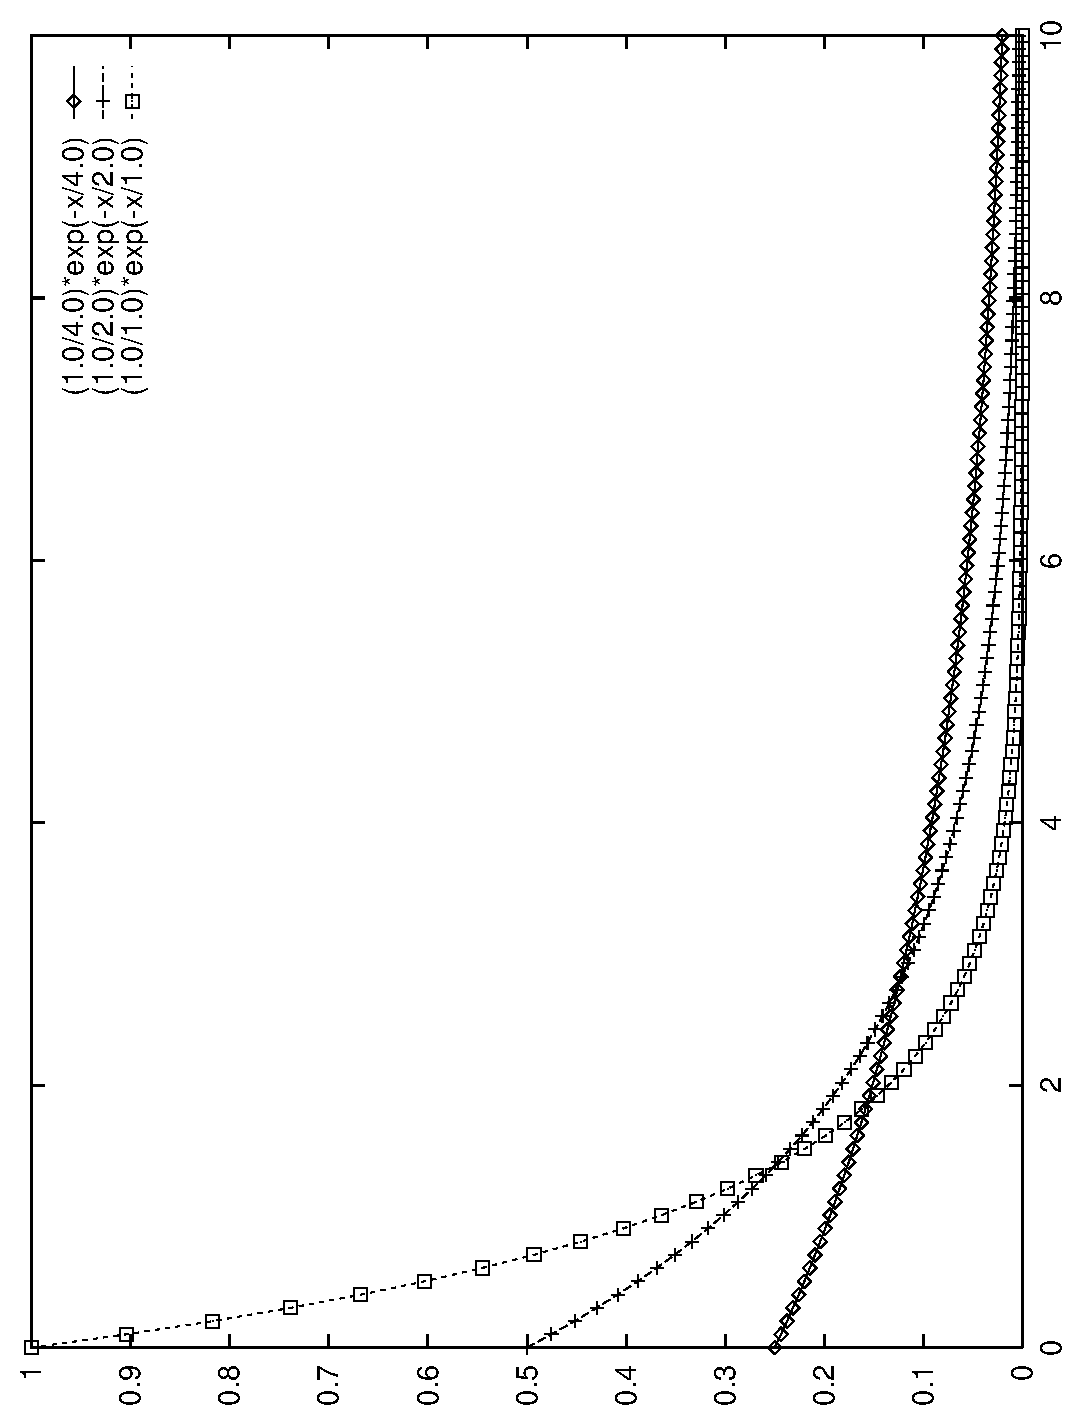
\includegraphics[height=12cm]{negexponential.eps}}\\
\caption{The Negative exponential distribution $a=1,2,4$.}
\end{figure}
\end{center}

\clearpage

\section{Internal Variables}

\begin{itemize}
\item pMean - The constant variable $a$ in the former equation.
\end{itemize}

%********************
\index{pMean (Variable)}
%********************

\vspace*{5mm}

\section{Public Methods}

\noindent
These methods can be used by all \cpp - programs, that have included the
header file NegExponential.h and the library EA. If you declare only
Population.h, we can't use these methods in this version.

\subsection{Constructors}

%---------------------------------------------------------------------------%
% 001
\index{NegExponential!( double mean )}
\setNormalInstance
\printMethodWithOneParam
{}
{NegExponential}
{double}
{mean}
{The constant variable $a$.}
{The default constructor. Generates the random generator of Negative
Exponential distribution.}
{None.}
{None.}
%---------------------------------------------------------------------------%

%---------------------------------------------------------------------------%
% 002
\index{NegExponential!( double mean, RNG\& r )}
\setNormalInstance
\setCorrectWidthThree{8pt}
\setParamOne{mean}{double}{The constant variable $a$.} 
\setParamTwo{r}{RNG\&}{RNG class}
\printMethodWithParamsSaved
{}
{None.}
{NegExponential}
{The constructor. Generates the random generator of Negative
Exponential distribution.}
{None.}
\setCorrectWidthThree{4pt}
%---------------------------------------------------------------------------%

\vspace*{5mm}

\subsection{Operators}

%---------------------------------------------------------------------------%
% 003
\index{operator( )!( double mean )} 
\setNormalInstance
\printMethodWithOneParam
{double}
{operator( )}
{double}
{mean}
{The constant variable $a$.}
{Gets the result of Negative Exponential distribution.}
{The result of Negative Exponential distribution.}
{None.}
%---------------------------------------------------------------------------%

\clearpage

%---------------------------------------------------------------------------%
% 004
\index{operator( )!( )} 
\setNormalInstance
\printEmptyMethodReturnSpecial
{double}
{operator( )}
{Gets the result of Negative Exponential  distribution.}
{The result of Negative Exponential distribution.}
{None.}
%---------------------------------------------------------------------------%

\vspace*{10mm}

\subsection{Information Retrieval Methods}

%---------------------------------------------------------------------------%
% 005
\index{mean!( )} 
\setConstInstance
\printEmptyMethodReturnSpecial
{double}
{mean}
{Returns the varible {\em pMean}.}
{The variable {\em pMean}.}
{None.}
%---------------------------------------------------------------------------%

%---------------------------------------------------------------------------%
% 006
\index{mean!( double newMean )} 
\setNormalInstance
\printMethodWithOneParam
{void}
{mean}
{double}
{newMean}
{New constant variable {\em pMean}.}
{Sets the constant variable {\em pMean} using new variable {\em newMean}.}
{None.}
{None.}
%---------------------------------------------------------------------------%

\vspace*{10mm}

\subsection{The probability}

%---------------------------------------------------------------------------%
% 007
\index{p!( const double\& x )} 
\setConstInstance
\printMethodWithOneParam
{double}
{p}
{const double\&}
{x}
{The factor which you want to calculate the probability.}
{Returns the probability of {\em x}.}
{The probability.}
{None.}
%---------------------------------------------------------------------------%



